% Q19：按固定候选 PDF 第 2 页重绘正三角形、中心、MN 与角 alpha；不表示精确比例。
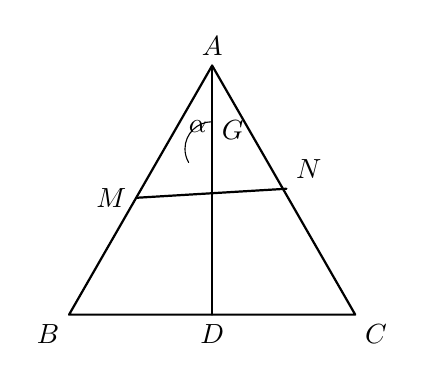
\begin{tikzpicture}[line cap=round,line join=round,scale=1.15]
  \coordinate (A) at (0,2.75);
  \coordinate (B) at (-1.58,0);
  \coordinate (C) at (1.58,0);
  \coordinate (D) at (0,0);
  \coordinate (G) at (0,1.83);
  \coordinate (M) at (-0.84,1.29);
  \coordinate (N) at (0.82,1.39);

  \draw[thick] (A)--(B)--(C)--cycle;
  \draw[thick] (A)--(D);
  \draw[thick] (M)--(N);
  \draw (G) ++(90:0.30) arc[start angle=90,end angle=210,radius=0.30];

  \node[above] at (A) {$A$};
  \node[below left] at (B) {$B$};
  \node[below right] at (C) {$C$};
  \node[below] at (D) {$D$};
  \node[above right] at (G) {$G$};
  \node[left] at (M) {$M$};
  \node[above right] at (N) {$N$};
  \node at (-0.16,2.08) {$\alpha$};
\end{tikzpicture}
